\documentclass[a4paper, 11pt, french]{report}
\usepackage[utf8]{inputenc}
\usepackage[francais]{babel}
\usepackage[T1]{fontenc}
\usepackage[colorlinks=true, urlcolor=blue, linkcolor=blue]{hyperref}
\usepackage{graphicx}
\usepackage{wrapfig}
\usepackage{multicol}

\title{IHM2 - Projet Caterpillar Scheduler}
\author{Robin Boncorps, Gwendal Daniel}
\date{\today}

\begin{document}
\maketitle

\renewcommand{\contentsname}{Sommaire} %renomme la table des matières
\tableofcontents

\chapter{Introduction} % au blaire
Ce projet nous a été donné comme projet de travaux pratiques pour le cours d'interface hommes-machines 2. L'objectif est de développer une application Android permettant de gérer, d'organiser et de sauvegarder une ou plusieurs listes de tâches. Le sujet impose un développement en Java, qui est le langage de développement sous Android.
\newline

~\\
Dans la liste des fonctionnalités impératives, on retrouve
\begin{itemize}
\item Gestion de listes
\item Gestion de tâches dans une liste
\item Sauvegarde et chargement
\end{itemize}
~\\

Il nous était en outre demandé de nous focaliser sur l'aspect interface graphique de l'application, le but étant d'offrir une interface simple d'utilisation et intuitive pour l'utilisateur. Cet utilisateur n'était pas nécessairement un informaticien mais n'importe quelle personne ayant besoin de gérer une liste de tâches.
\newline

Le présent rapport s'articulera autour de deux axes majeurs : la modélisation et l'implémentation. Dans un premier temps nous détaillerons la modélisation retenue, les scénarios d'utilisation que nous souhaitions mettre en place, ainsi que le storyboard général de l'application. Ensuite, nous nous pencherons sur la phase d'implémentation, expliquerons la structure des widgets retenue, ainsi que les différents tests ayant ammené l'application à évoluer.

\chapter{Modélisation}
		\section{Storyboarding} %robin
Le storyboarding est la première phase de modélisation lorsque l'on décide de concevoir une interface utilisateur. Il consiste en un petit résumé visuel de l'utilisation générale de l'application. Nous nous somme concentré sur la vision utilisateur dans le storyboard. Nous avons voulu montrer l'apport au quotidien de l'utilisation de \emph{Caterpillar Scheduler}, ce storyboard est évidemment transposable à d'autres situations.

\section{Scenarios} % robin
Cette section détaillera l'ensemble des scénarios que nous avons utilisé durant la modélisation et le développement de l'application. Ces scénarios nous on permis d'une part de déterminer les fonctionnalités que nous souhaitions proposer, et ont servi de ligne directrice pour les phases de tests. Il était donc important d'avoir une liste à la fois complète et suffisament détaillée pour un utilisateur externe.
\newline

Les scénarios seront présentés par ordre de complexité, nous montrerons dans un premier temps les scénarios de base comme la validation ou la création de tâche, puis nous poursuivrons avec les scénarios plus complexes.
\newline
Un scénario d'utilisation complet sera également donné.
\newline

Lors des tests des différents scénarios, nous n'avons, dans un premier temps, donné que l'intitulé du scénario, afin de voir si notre application était suffisament ergonomique et intuitive pour permettre de le réaliser sans plus de détails. Dans un second temps, nous avons explicité les différentes actions à effectuer afin de tester les fonctionnalités à proprement parler.
\newline

~\\
\textbf{Création de listes :} 
\begin{enumerate}
	\item Cliquer sur la zone de texte qui permet d'ajouter une liste
	\item Renseigner le nom de la liste à ajouter
	\item Valider en cliquant sur "Done" dans le clavier android
\end{enumerate}
~\\
\textbf{Creation de tâches attachées à une liste :} 
\begin{enumerate}
	\item Cliquer sur la liste précédemment créée (voir le scénario associé)
	\item Cliquer sur la zone de texte qui permet d'ajouter une tâche
	\item Renseigner le nom de la tâche à ajouter
	\item Valider en cliquant sur "Done" dans le clavier android
\end{enumerate}


Ce scénario ressemble beaucoup au scénario de création de liste, ce qui est normal et souhaité : nous voulions que les différentes actions soient accessibles de la même manière, afin de ne pas perturber l'utilisateur.

~\\
\textbf{Validation de tâche : }
\begin{enumerate}
	\item Cliquer sur la tâche que l'on souhaite valider
\end{enumerate}

~\\
\textbf{Suppression de tâche ou de liste : } dans l'optique de rendre l'utilisation de l'application simple, la procédure de suppression est la même pour les listes et les tâches.
\begin{enumerate}
	\item Faire un appui long sur la liste/tâche à supprimer.
	\item Cliquer sur "Delete" sur le menu contextuel.
\end{enumerate}

Nous noterons qu'aucune confirmation n'est demandée. Ceci découle du fait qu'il faille faire un appui long pour accéder au menu contextuel, qui n'est pas une action que l'on pourrait faire sans le vouloir.

~\\
\textbf{Renommage de tâche ou de liste : } dans l'optique de rendre l'utilisation de l'application simple, la procédure de renommage est la me pour les listes et les tâches.
\begin{enumerate}
	\item Faire un appui long sur la liste/tâche à renommer.
	\item Cliquer sur "Rename" sur le menu contextuel.
	\item Cliquer sur la zone de texte qui permet de rentrer le nouveau nom de la liste/tâche.
	\item Valider la saisie en cliquant sur "OK" dans le clavier android.
	\item Valider le renommage en cliquant sur "Rename" dans le formulaire.
\end{enumerate}

~\\
\textbf{Scénario complet : } Ce scénario nous a servi de scénario référence pour tester l'application dans son ensemble. Il comprend la création d'une liste contenant une tâche qui sera valider par la suite. Nous ne presenterons pas le renommage ou la suppression dans ce scenario car ces actions ne font pas partie du flot nominal.
\begin{enumerate}
	\item Créer une liste.
	\item Cliquer sur la liste pour accéder à ses tâches.
	\item Créer une tâche.
	\item Cliquer sur la tâche pour la valider.
\end{enumerate}
Tous les scénarios présentés sont simples, ceci pour garantir une appropriation facile de l'application par n'importe quel utilisateur.

\section{Noyau}

Cette section abordera le fonctionnement interne de l'application : le noyau. Nous nous intéresserons à la modélisation retenue ainsi qu'aux différentes fonctionnalités que nous souhaitions développer. Enfin, nous traiterons de l'influence de ce noyau sur la réalisation de l'interface, des facilités et des difficultés d'utilisation que nous avons rencontré lors de son utilisation.
\newline

Il est à noter que nous ne nous sommes pas focalisés sur le développement du noyau de l'application, mais plutôt sur l'aspect graphique et l'ergonomie. Néanmoins, nous pensons qu'un modèle "solide" permet de fournir des informations claires à l'utilisateur (par exemple en cas d'action non réalisable) et participe ainsi à l'ergonomie générale du logiciel.

\subsection{Structure}

Le noyau est découpé en deux partie :
	\begin{itemize}
		\item Les classes qui représentent les listes et les tâches
		\item La gestion de la base de données.
	\end{itemize}
Nous détaillerons ici les choix d'implémentation retenus pour ces deux parties.

\subsubsection{Les classes représentant les listes et tâches}

Une liste est composé de : 
\begin{itemize}
	\item Un identifiant unique
	\item Un nom
\end{itemize}
~\\
~\\
~\\
Une tâche est composé de : 
\begin{itemize}
	\item Un identifiant unique
	\item Un nom
	\item un état de validation
	\item l'identifiant de la liste à laquelle elle est rattachée.
\end{itemize}
~\\

Ces deux classes correspondent à leur représentation en base de données.
Tous les attributs sont privées et peuvent être modifiés ou retournés grâce à des setteurs et getteurs.
	
\subsubsection{La gestion de la base de données}

Une base de données est essentielle si l'on souhaite que les données fournies par l'utilisateur soient persistantes lors de la fermeture de l'application.
Android utilise SQLite pour la gestion de la base de données.

Les données qui doivent persister sont : 
\begin{itemize}
	\item Les listes
	\item Les tâches
\end{itemize}

La base sera donc composée de deux tables :
	\begin{figure}[!h]
		\centering
		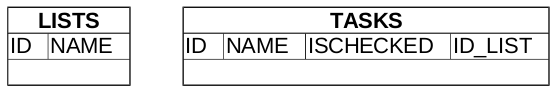
\includegraphics[scale=0.5]{Tables.png}
		\label{Tables SQL}
	\end{figure}

On notera que le champ ID\_LIST est une clé étrangère qui correspond à l'identifiant de la liste à laquelle appartient la tâche

\subsection{Fonctionnalités}
Le noyau représente les données de l'application. Il offre donc plusieurs fonctionnalités qui devront pouvoir être accessibles dans l'interface graphique.Voici toutes les fonctionnalités accessibles :
	\begin{itemize}
		\item Ajout/Suppression de listes
		\item Ajout/Suppression de tâches
		\item Renommage de liste/de tâche
		\item Validation/Invalidation de tâche
		\item Affichage des tâches non validées en premier
		\item Affichage du nombre de tâches restant à valider dans une liste
		\item Suppression de toutes les listes dont toutes les tâches ont été validées (accès par un menu)
	\end{itemize}

\chapter{Implémentation}
Après la modélisation vient l'implémentation. Nous avons donc utilisé Java pour Android pour developper cette application. 

\section{Organisation générale} % gwendal
L'application se compose de 2 activités Android, une pour la gestion des listes et une pour la gestion des tâches.

\subsection{ListActivity} % gwendal
Cette activité permet de gérer les listes.
	\subsubsection{Layout}
	Cette activité s'appuie sur une représentation graphique (layout) qui comprend : 
	\begin{itemize}
		\item Une ListView qui contient toutes les listes
		\item Un TextEdit qui permet de renseigner le nom de la liste à ajouter
	\end{itemize}
	~\\
	Une ListView contient une liste d'éléments identiques. Nous avons choisi de représenter une liste (un élement) par un TextView, qui permet d'afficher du texte.Une particularité des TextView permet d'afficher des images sur les cotés du widget. Ceci est utilisé pour ajouter une icone réprésentant une liste sur la gauche de l'élément, ainsi que le nombre de tâches restant à valider sur la droite.
	
	Le TextEdit permet, lors du clic sur celui-ci, d'afficher le clavier pour saisir le nom de la nouvelle liste. La couleur de fond a été modifée pour permettre de bien le différencier d'avec la ListView. Nous avons aussi choisi d'ajouter une image pour que l'utilisateur identifie bien l'utilité du champ de saisie.
	
	\subsubsection{Spécificités}
	A cette représentation visuel, il faut ajouter des actions. 
	La première chose est de récupérer les listes dans la base de données. Il faut ensuite les ajouter dans un adapter.
	Cet adapter permet de créer un widget par liste selon le layout vu au dessus et de les ajouter les uns à la suite des autres dans la ListView (un conteneur). Lors de la création du widget de liste, une requete sql est effectué pour connaître le nombre de tâches qu'il reste à valider dans la liste. Cette information est ensuite ajouter en tant que Drawable dans la partie droite du widget.
	Aussi, l'appui sur "Done" sur le clavier Android ajoute une liste automatiquement. Ceci aurait pu être fait grâce à un boutton placé à côté du champ mais il apparaissait plus intuitif d'ajouter ce comportement. L'ajout est fait directement en base de données, ce qui met à jour le contenu de l'adapter.
	Il est important de noter que chaque action sur les listes est répercuté directement sur la base de données pour garder un état cohérent, et garantir la reprise en l'état si l'application est fermée.
	
	L'appui sur une liste lance un Intent qui permet d'afficher la liste des tâches spécifique à la liste cliquée (identifiant et nom de la liste sont passé en paramètre).
	
\subsection{TaskActivity}
Cette activité permet de gérer les tâches spécifiques à une liste donnée.
	\subsubsection{Layout}
	Cette activité s'appuie sur une représentation graphique (layout) qui comprend : 
	\begin{itemize}
		\item Un TextEdit qui permet de renseigner le nom de la tâche à ajouter
		\item Une ListView qui contient toutes les tâches
	\end{itemize}
	~\\
	Une tâche est représenter par une CheckedTextView, widget qui permet d'afficher du texte ainsi qu'une Checkbox.
	L'ordre des widgets à été changé par rapport à la première activité pour permettre de différencier les deux vues facilement. De plus le titre de la vue tâche correspond au nom de la liste qui contient les tâches. 
	
	\subsubsection{Spécificités}
	Les actions disponibles sont les memes que pour les listes. Cependant, l'appui sur une tâche entraîne la validation de celle-ci (la checkbox est cochée) ainsi que le déplacement de la tâche en fin de liste, avec les tâches déjà validées.
	L'ordre des tâches en base de données reste le même (dans l'ordre d'ajout) mais seul l'ordre dans lequel sont affichées les tâches change. Ainsi, lors de la dévalidation d'une tâche, elle retrouve sa place entre les tâches qui ne sont pas validées.



\section{Tests}
Nous avons effectué plusieurs séances de tests au cours des phases de développement. Nous avons aussi fait tester notre application par des personnes extérieures pour avoir un nouveau regard. Dans l'ensemble, les tests des différentes fonctionnalités se sont avérés concluant. 
L'ajout et la suppression de listes et de tâches s'est avéré intuitif comme nous l'espérions. 
Néanmoins, quelques fonctionnalités ont posé problème. 
Tout d'abord , la procédure de renommage de tâches et de listes n'a pas bien été comprise par les utilisateurs extérieurs. Nous avons donc changer la procedure pour correspondre à leurs attentes.
Ensuite, certaines fonctionnalités manquaient, notamment le ré-ordonnancement des tâches validées. Nous avons donc pallier à tous les manques retenus pour avoir une application compléte et simple à utiliser.


\chapter{Conclusion} 
Pour conclure, nous avons mené à bien l'essentiel des fonctionnalités que nous avions prévu. Nous sommes un peu déçu de n'avoir pas pu avoir le temps de faire notre propre design d'interface graphique (personnalisation des widgets de tâches,...) par manque de temps. En effet, android est parfois compliqué à prendre en main.
\newline

Ce projet nous a permis d'entrevoir les nombreuses possibilités du développement sous Android et permis de faire un premier pas dans ce monde. Le fait que l'on puisse avoir sur son smartphone, une application "maison" est une grande fierté. 

L'application en l'état est parfaitement utilisable et nous allons l'utiliser en cette fin de semestre pour faire une liste de toutes les tâches qu'il nous reste à faire.
\newline

Nous tenons également à remercier Guillemette et Morgane, pour leur tests et conseils avisés, ainsi que pour l'icône de l'application.

\end{document}
